\documentclass[11pt]{article}

\usepackage[T1]{fontenc}
\usepackage[utf8]{inputenc}
\usepackage{amsmath,amssymb,amsthm,mathtools}
\usepackage{mathpartir}
\usepackage{stmaryrd}
\usepackage{enumitem}
\usepackage{graphicx}
\usepackage{tikz}
\usetikzlibrary{arrows.meta,fit,positioning}
\usepackage[colorlinks=true,linkcolor=blue!55!black,urlcolor=blue!55!black]{hyperref}
\usepackage[margin=1in]{geometry}
\usepackage{xcolor}

\newtheorem{definition}{Definition}[section]
\newtheorem{lemma}[definition]{Lemma}
\newtheorem{theorem}[definition]{Theorem}
\newtheorem{corollary}[definition]{Corollary}
\newtheorem{proposition}[definition]{Proposition}
\theoremstyle{remark}
\newtheorem{remark}[definition]{Remark}

\newcommand{\leanfile}[1]{\footnote{Lean formalization: \texttt{Crush/Metatheory/#1}.}}
\newcommand{\leanfiles}[1]{\footnote{Lean formalization: \texttt{Crush/Metatheory/#1}.}}
\newcommand{\leanpaths}[1]{\footnote{Lean source: \texttt{#1}.}}
\newcommand{\sectioncontents}[1]{%
  \smallskip\noindent\textbf{Contents of this section.} #1\par\medskip}
\newcommand{\Bool}{\mathsf{Bool}}
\newcommand{\Base}{\mathsf{Base}}
\newcommand{\Fn}{\mathsf{Fn}}
\newcommand{\clos}{\mathsf{clos}}
\newcommand{\app}{\mathsf{app}}
\newcommand{\den}[3]{\llbracket #1\rrbracket_{#2,#3}}
\newcommand{\erase}[1]{\lfloor #1\rfloor}
\newcommand{\unary}[1]{\mathcal D\llbracket #1\rrbracket}
\newcommand{\flattr}[1]{\mathcal F\llbracket #1\rrbracket}
\newcommand{\smtenc}[2]{\mathcal A\llbracket #2\rrbracket[#1]}
\newcommand{\guardenc}[2]{\mathcal G\llbracket #2\rrbracket[#1]}
\newcommand{\sat}{\models}
\newcommand{\satt}{\models^{\mathsf T}}
\newcommand{\smtsat}{\models_{\mathsf{SMT}}}
\newcommand{\unsat}{\mathsf{Unsat}}
\newcommand{\Gen}{\mathsf{Gen}}
\newcommand{\Theory}{\mathsf{Theory}}
\newcommand{\Theorys}[1]{\mathsf{Theory}^{\!*}(#1)}
\newcommand{\Commands}{\mathsf{Commands}}
\newcommand{\Rep}{\mathsf{Rep}}
\newcommand{\SameCmd}{\mathrel{\equiv_{\mathsf{cmd}}}}
\newcommand{\Lawful}{\mathsf{Lawful}}
\newcommand{\Val}{\mathsf{Val}}
\newcommand{\WF}{\mathsf{WF}}
\newcommand{\args}{\mathsf{args}}
\newcommand{\res}{\mathsf{res}}
\newcommand{\FV}{\mathsf{FV}}

\title{The Metatheory of Crush's Certified Lowering Pipeline}
\author{lean-crush}
\date{August 2026}

\begin{document}
\maketitle

\begin{abstract}
Crush translates a supported finite collection of Lean propositions into SMT
commands. This document explains the current mathematical framework for that
translation: intrinsically typed higher-order syntax, datatype-aware source
models, total flattened defunctionalization, raw SMT command semantics, native
datatype declarations, guarded carrier encodings, and exact agreement with a
completed production command snapshot. It is written in dependency order:
each object and notation is introduced before the first theorem that uses it.
The final theorem justifies the reified higher-order theory and the exact
semantic command set produced by the modeled lowering pipeline; it does not
assume that an external solver is correct and does not assign a denotation to
arbitrary \texttt{Lean.Expr}.
\end{abstract}

\tableofcontents

\section{Reader's guide}
\sectioncontents{The question answered by the formalization; proof stages; notation and scope.}

\subsection{What is being proved}

The formalization studies this pipeline:
\begin{center}
\resizebox{0.98\linewidth}{!}{$
\boxed{\text{supported Lean fact array}}
\longrightarrow
\boxed{\text{intrinsically typed HO theory}}
\longrightarrow
\boxed{\text{combined flattened FO theory}}
\longrightarrow
\boxed{\text{semantic raw command set}}
$}
\end{center}
The first arrow is a partial recognizer: every accepted fact is reified under
one common signature and datatype environment, and unsupported Lean syntax is
rejected. The remaining intrinsic transformations are total. Native datatype
commands and recursive well-formedness definitions are modeled components of
the final command set. The principal semantic conclusion is:

\begin{quote}
If the completed represented command set is semantically unsatisfiable, then
the reified higher-order source theory is unsatisfiable in every source model
satisfying the retained datatype laws.
\end{quote}

The proof is by countermodel construction. Starting from one lawful model of
the complete higher-order theory, Lean constructs one model of all flattened
sentences and generated obligations, then constructs one relational SMT model
satisfying native declarations, derived recursive guards, ordinary
declarations, and assertions. Contraposition yields the desired reflection of
unsatisfiability.

\subsection{Proof stages}

The argument is organized into seven stages:
\begin{enumerate}[leftmargin=*,label=\arabic*.]
  \item Define an intrinsically typed higher-order source language and its
        ordinary function-space semantics.
  \item Describe productive monomorphic datatype blocks, their finite
        free-algebra semantics, and the source-model lawfulness contract.
  \item Define an intrinsically typed first-order target whose function-value
        sorts are opaque, then give total flattened defunctionalization.
  \item Interpret every translated sentence in one canonical model and prove
        simultaneous validity of the aggregate target theory.
  \item Give raw semantics to the admitted SMT command fragment and prove one
        exact command-set representation theorem.
  \item Lift guarded and datatype carriers, validate native datatype and
        recursive guard commands, and combine all components in one raw model.
  \item Retain structural Lean reification, exact stateful VCG execution, and
        proof-producing agreement with a completed production snapshot.
\end{enumerate}

\subsection{Metavariables and notation}

The following metavariables are used consistently throughout the document.
Semantic and translation notation is introduced later, beside the definition
that gives it meaning.
\[
\begin{array}{c@{\quad}l}
 e,f,a & \text{source or target terms; $f$ is usually function-valued},\\
 \varphi,\psi & \text{Boolean formulas; a closed formula is a sentence},\\
 \Phi & \text{a finite higher-order source theory},\\
 \beta & \text{an opaque source base-sort name},\\
 \alpha,\gamma,\sigma,\tau,\upsilon & \text{source types},\\
 \kappa & \text{a first-order sort},\\
 \Gamma,\Delta & \text{typing contexts},\\
 \Sigma & \text{a typed signature},\\
 T & \text{a typed first-order theory},\\
 M,N & \text{semantic models},\\
 \rho & \text{a source valuation or typed renaming},\\
 \nu & \text{a target valuation},\\
 v,w & \text{individual semantic values},\\
 \mathcal E & \text{a concrete FO-to-SMT encoding choice},\\
 \mathcal G & \text{a guard-aware SMT encoding choice},\\
 C & \text{an ordered array of raw SMT commands}.
\end{array}
\]
Subscripts $s$, $t$, and $q$ mean source, typed target, and raw SMT model,
respectively. Proof-facing Lean declarations use the corresponding Greek
binders; executable allocation and state code keeps descriptive names when
several objects have the same mathematical role.

\section{The intrinsically typed higher-order source}
\sectioncontents{Types, contexts, terms, and ordinary higher-order semantics.}

\subsection{Types, contexts, and signatures}

\begin{definition}[Source types]
Let $\beta$ range over opaque base-sort names. Source types are generated by
\[
  \tau ::= \Bool \mid \Base(\beta) \mid \tau\to\sigma.
\]
Arrows are nondependent and associate to the right. A context
$\Gamma=[\tau_0,\ldots,\tau_{n-1}]$ records local binders with the newest binder
at the head. We write $\Gamma,\tau$ for extension by a new binder of type
$\tau$; this is stored as $\tau::\Gamma$ in Lean. A signature $\Sigma$ is a list
of the types of global constants.
\leanfile{HO/Core.lean}
\end{definition}

We write $\Gamma\ni\tau$ for the intrinsically typed lookup judgment. Its
inhabitants are de Bruijn references, generated by:
\begin{mathpar}
 \inferrule*{ }
   {Z:\Gamma,\tau\ni\tau}
 \qquad
 \inferrule*{i:\Gamma\ni\tau}
   {S\,i:\Gamma,\sigma\ni\tau}.
\end{mathpar}
The judgment is intrinsically witnessed: its derivation simultaneously records
the position and proves the type at that position. The witness $Z$ denotes
index zero and $S\,i$ denotes the successor of the index denoted by $i$.
Forgetting the derivation yields the natural-number index used when collecting
free variables.
Constants use the same typed-reference representation in $\Sigma$. Therefore a
variable or constant with the wrong type cannot be constructed.

For $i:\Gamma\ni\tau$, write $x_i$ for the local-variable term selected by
$i$. For $k:\Sigma\ni\tau$, write $c_k$ for the global-constant term selected
by $k$ from the signature. The subscripts are typed lookup witnesses, not
variable or constant names.

\begin{definition}[Source terms]
The intrinsic judgment $\Sigma;\Gamma\vdash e:\tau$ has variables, constants,
Boolean literals and connectives, same-type equality, lambda, application, and
universal and existential quantification:
\begin{mathpar}
 \inferrule{i:\Gamma\ni\tau}
   {\Sigma;\Gamma\vdash x_i:\tau}
 \qquad
 \inferrule{k:\Sigma\ni\tau}
   {\Sigma;\Gamma\vdash c_k:\tau}

 \inferrule{\Sigma;\Gamma,\tau\vdash e:\sigma}
   {\Sigma;\Gamma\vdash\lambda x{:}\tau.e:\tau\to\sigma}
 \qquad
 \inferrule{\Sigma;\Gamma\vdash f:\tau\to\sigma\\
             \Sigma;\Gamma\vdash a:\tau}
   {\Sigma;\Gamma\vdash f\,a:\sigma}

 \inferrule{\Sigma;\Gamma\vdash e_1:\tau\\
             \Sigma;\Gamma\vdash e_2:\tau}
   {\Sigma;\Gamma\vdash e_1=e_2:\Bool}
 \qquad
 \inferrule{\Sigma;\Gamma,\tau\vdash\varphi:\Bool\\Q\in\{\forall,\exists\}}
   {\Sigma;\Gamma\vdash Qx{:}\tau.\varphi:\Bool}.
\end{mathpar}
The omitted rules are the standard typed Boolean rules. A formula is a term of
type $\Bool$; a sentence is a formula in the empty context.
\leanfile{HO/Core.lean}
\end{definition}

Quantifiers may range over arrow types. Thus the modeled language is genuinely
higher-order even though its arrows are nondependent.

\subsection{Source models}

\begin{definition}[Source type denotation]
A carrier family $B$ assigns a nonempty type $B(\beta)$ to each opaque base
sort. Its extension to source types is
\[
 \llbracket\Bool\rrbracket_B=\mathsf{Prop},\qquad
 \llbracket\Base(\beta)\rrbracket_B=B(\beta),\qquad
 \llbracket\tau\to\sigma\rrbracket_B=
   \llbracket\tau\rrbracket_B\to\llbracket\sigma\rrbracket_B.
\]
Thus the only choices in $B$ are the carriers assigned to opaque base sorts.
\end{definition}

\begin{definition}[Source model and valuation]
A source model $M_s$ consists of a carrier family $B$ and an interpretation
$c_k^{M_s}\in\llbracket\tau\rrbracket_B$ for each
$k:\Sigma\ni\tau$. A
valuation $\rho$ for $\Gamma$ assigns a value in
$\llbracket\tau\rrbracket_B$ to every $i:\Gamma\ni\tau$. We write $\rho[v]$
for extension by a new head value $v$.
\end{definition}

\begin{definition}[Source denotation]
Denotation is structural. Variables use $\rho$, constants use $M_s$, and the
Boolean forms have their ordinary meanings. From this point onward,
\[
  \den{e}{M_s}{\rho}
\]
denotes the value of $e$ in $M_s$ under
$\rho$.\leanfile{HO/Semantics.lean} The higher-order clauses are
\[
\begin{aligned}
 \den{\lambda x{:}\tau.e}{M_s}{\rho}
   &=\lambda v.\den{e}{M_s}{\rho[v]},\\
 \den{f\,a}{M_s}{\rho}
   &=\den{f}{M_s}{\rho}(\den{a}{M_s}{\rho}),\\
 \den{\forall x{:}\tau.\varphi}{M_s}{\rho}
   &=\forall v\in\llbracket\tau\rrbracket_B,
       \den{\varphi}{M_s}{\rho[v]},\\
 \den{\exists x{:}\tau.\varphi}{M_s}{\rho}
   &=\exists v\in\llbracket\tau\rrbracket_B,
       \den{\varphi}{M_s}{\rho[v]}.
\end{aligned}
\]
\end{definition}

\begin{definition}[Sentences, theories, and satisfaction]
A source sentence is a Boolean term in the empty context. A finite source
theory is a list $\Phi=[\varphi_1,\ldots,\varphi_n]$ of sentences sharing one
signature $\Sigma$. We introduce the satisfaction notation
\[
\begin{aligned}
 M_s\sat\varphi
   &\quad\Longleftrightarrow\quad
     \den{\varphi}{M_s}{\varnothing},\\
 M_s\satt\Phi
   &\quad\Longleftrightarrow\quad
     \forall\varphi\in\Phi.\;M_s\sat\varphi,
\end{aligned}
\]
where $\varnothing$ is the unique valuation of the empty context.
\leanfile{HO/Semantics.lean}
\end{definition}

\begin{definition}[Source unsatisfiability]
Sentence and theory unsatisfiability are semantic properties:
\[
\begin{aligned}
 \unsat_{\mathsf{HO}}(\varphi)
   &\quad\Longleftrightarrow\quad
     \forall M_s.\;\neg(M_s\sat\varphi),\\
 \unsat_{\mathsf{HO}}(\Phi)
   &\quad\Longleftrightarrow\quad
     \forall M_s.\;\neg(M_s\satt\Phi).
\end{aligned}
\]
For a proof-relevant model contract $\mathcal L(M_s)$, the restricted form is
\[
 \unsat_{\mathsf{HO}}^{\mathcal L}(\Phi)
 \quad\Longleftrightarrow\quad
 \forall M_s.\;\forall \ell:\mathcal L(M_s).\;
   \neg(M_s\satt\Phi).
\]
The Lean definitions are \texttt{Unsatisfiable},
\texttt{TheoryUnsatisfiable}, and \texttt{UnsatisfiableUnder}.
\leanfile{HO/Semantics.lean}
\end{definition}

\section{Datatype-aware source semantics}
\sectioncontents{Intrinsic mutual blocks; finite free values; source-symbol ownership; lawful model environments.}

Native datatype lowering strengthens the class of source models without
changing the HO term language. Constructors, selectors, and testers remain
ordinary constants in $\Sigma$; a separate typed description says which
constants they are and what laws their interpretations obey.

\subsection{Intrinsic datatype blocks}

\begin{definition}[Mutual datatype block]
Fix an arity $n>0$. A field sort is either an external base sort or a direct
reference to one of the $n$ datatypes:
\[
 q ::= \mathsf{base}(\beta)\mid\mathsf{data}(d),
 \qquad d\in\mathsf{Fin}(n).
\]
A field declaration pairs a descriptive name with $q$; a constructor is a
name and an ordered field list; a datatype declaration is a base-sort identity
and an ordered constructor list. A block $B$ assigns one datatype declaration
to every $d\in\mathsf{Fin}(n)$. Typed positions, rather than names, identify
members. After this definition we write
\[
 B\vdash_D d,\qquad B\vdash_C[d]K,\qquad K\vdash_F F
\]
for a datatype position, a constructor position in $d$, and a field position
in $K$, respectively. These correspond to Lean's scoped notations
\texttt{B~$\vdash$\textsuperscript{D}},
\texttt{B~$\vdash$\textsuperscript{C}[d]~K}, and
\texttt{K~$\vdash$\textsuperscript{F}~F}.
\leanfile{Datatype/Core.lean}
\end{definition}

\begin{definition}[Block well-formedness]
A block is structurally well formed when it is nonempty, its datatype
base-sort identities are pairwise distinct, and every field classified as
external is fresh from those datatype identities. Direct recursive fields can
refer only to the current block, so unsafe cross-block cycles are not
representable. The executable predicate \texttt{wellFormed} is proved
equivalent to this proposition.
\leanfile{Datatype/Core.lean}
\end{definition}

\subsection{Finite free values}

\begin{definition}[Canonical datatype values]
For external carriers $B_0(\beta)$, the family
$\Val_B(B_0,d)$ and its heterogeneous constructor arguments are defined
mutually. A value has exactly one finite constructor tree:
\[
 v ::= K(a_1,\ldots,a_m),
\]
where an external field contains an element of $B_0(\beta)$ and a recursive
field contains another value $v'\in\Val_B(B_0,d')$. The height of a value is
one plus the maximum height of its recursive fields. A block is
\emph{productive} when every $d$ has a finite value after all external
carriers are replaced by the unit type.
\leanfile{Datatype/Semantics.lean}
\end{definition}

\begin{theorem}[Free-algebra laws]
Canonical values satisfy constructor injectivity and disjointness,
constructor exhaustiveness, matching tester equations, matching selector
equations, and strict height decrease along every recursive field. Selectors
are total; on a nonmatching constructor their fallback is intentionally
unconstrained.
\leanfile{Datatype/Semantics.lean}
\end{theorem}

\subsection{Lawful source models}

\begin{definition}[Datatype symbol ownership]
For a block $B$ and source signature $\Sigma$, an ownership map
$\mathsf{Symbols}(\Sigma,B)$ selects the ordinary HO constants used as each
constructor, selector, and tester. The types of those constants are computed
from the block: constructor fields form a curried arrow telescope, selectors
map a datatype carrier to one field carrier, and testers return $\Bool$.
\leanfiles{Datatype/Syntax.lean and Datatype/Model.lean}
\end{definition}

\begin{definition}[Lawful datatype model]
Let $S:\mathsf{Symbols}(\Sigma,B)$. A witness
$\Lawful_B(S,M_s)$ contains an isomorphism
\[
 M_s.B(d.\mathsf{sort})\cong\Val_B(M_s.B,d)
\]
for every datatype position $d$, identifies every owned constructor with its
canonical curried interpretation, requires matching selectors to recover the
selected field, and requires each tester to recognize exactly its constructor.
Such a witness implies productivity of $B$.
\leanfile{Datatype/Model.lean}
\end{definition}

\begin{definition}[Datatype environment]
An environment $\mathcal D=[(B_1,S_1),\ldots,(B_k,S_k)]$ is an ordered list
of blocks and their ownership maps in one shared signature. The judgment
$\Lawful_{\mathcal D}(M_s)$ supplies a lawful witness for every entry. We write
\[
 \unsat_{\mathsf{HO}}^{\mathcal D}(\Phi)
 \quad\Longleftrightarrow\quad
 \forall M_s.\;\forall\ell:\Lawful_{\mathcal D}(M_s).\;
   \neg(M_s\satt\Phi).
\]
The empty environment recovers ordinary source unsatisfiability.
\leanfile{Datatype/Model.lean}
\end{definition}

\section{The intrinsically typed first-order target}
\sectioncontents{Erased sorts, abstract symbol families, target terms, and target models.}

\begin{definition}[First-order sorts and erasure]
Target sorts are
\[
 \kappa ::= \Bool\mid\Base(\beta)\mid\Fn(\tau,\sigma).
\]
Erasure is defined by
\[
 \erase{\Bool}=\Bool,\qquad
 \erase{\Base(\beta)}=\Base(\beta),\qquad
 \erase{\tau\to\sigma}=\Fn(\tau,\sigma).
\]
The last sort is opaque: it is not a function space in an arbitrary target
model. Context erasure maps every entry pointwise.
\leanfile{FO/Core.lean}
\end{definition}

\begin{definition}[Declarations and symbol families]
A declaration
\[
 d=(\kappa_1,\ldots,\kappa_n;\kappa)
\]
records an ordered argument telescope
$d.\mathsf{args}=[\kappa_1,\ldots,\kappa_n]$ and a result sort
$d.\mathsf{result}=\kappa$. Let $\mathsf{Decl}$ be the type of all such
declarations. A \emph{symbol family} is a declaration-indexed family of types
\[
 S:\mathsf{Decl}\longrightarrow\mathbf{Type},
 \qquad d\longmapsto S(d).
\]
An inhabitant $p:S(d)$ is one symbol identity whose declaration is exactly
$d$. The fiber $S(d)$ may contain no symbols, one symbol, or several distinct
symbols with the same argument and result sorts. Thus the declaration is part
of a symbol's type, while its identity remains separate from its declaration.
\leanfile{FO/Family.lean}
\end{definition}

\begin{definition}[Typed family arguments and symbol application]
Terms and heterogeneous argument vectors are defined mutually. For a context
$\Gamma$, the argument-vector family follows the declaration telescope:
\[
\begin{aligned}
 \mathsf{Args}_S(\Gamma,[])&=\{()\},\\
 \mathsf{Args}_S(\Gamma,\kappa_1::\bar\kappa)
   &=\{t\mid S;\Gamma\vdash t:\kappa_1\}
     \times\mathsf{Args}_S(\Gamma,\bar\kappa).
\end{aligned}
\]
The only general symbol-application rule is
\begin{mathpar}
 \inferrule{p:S(d)\\
             \bar t:\mathsf{Args}_S(\Gamma,d.\mathsf{args})}
   {S;\Gamma\vdash p(\bar t):d.\mathsf{result}}.
\end{mathpar}
Consequently the result sort and the complete ordered list of argument sorts
are determined by the index $d$. A missing, extra, or incorrectly sorted
argument cannot be represented. In particular, symbols are always fully
applied; partial application is not a target-language operation.
\end{definition}

For example, let $d=(\kappa_1,\kappa_2;\kappa)$ and let $p,q:S(d)$ be distinct
symbols. Given $S;\Gamma\vdash u:\kappa_1$ and
$S;\Gamma\vdash v:\kappa_2$, both $p(u,v)$ and $q(u,v)$ have sort $\kappa$,
but they remain different terms. Neither $p(u)$ nor $p(v,u)$ is constructible.

\begin{definition}[Target terms]
For a symbol family $S$, the intrinsic judgment $S;\Gamma\vdash t:\kappa$
contains variables, the fully applied family symbols above, Boolean literals
and connectives, same-sort equality, and first-order quantifiers. It contains
neither lambda nor a distinguished higher-order application constructor. A
function value is merely an element of an opaque $\Fn(\tau,\sigma)$ carrier;
applying that value later requires an ordinary family symbol with the appropriate
declaration.
\leanfiles{FO/Family.lean and FO/FamilySemantics.lean}
\end{definition}

\paragraph{Why translation uses a family.}
The finite target syntax also exists: a finite signature is a list
$\Xi=[d_0,\ldots,d_m]$, and a symbol occurrence carries a typed position
showing that some $d_j$ is its declaration. That form is useful after allocation,
but inconvenient during recursive translation. A recursive branch may discover
a new closure or application symbol; combining two branches then concatenates
their declaration traces. If terms already stored numeric signature positions,
those positions would have to be weakened and reindexed after every such
concatenation.

With a family, the translator instead constructs a structural identity
$p:S(d)$ immediately. Recursive results concatenate an occurrence trace of
existential packages $(d,p)$, while already constructed terms remain unchanged.
For flattened defunctionalization, $S$ is an indexed inductive family whose
constructors represent source constants, application symbols, and closures.
Each constructor's result index is its exact declaration; the flattened symbol
definition below spells out those shapes.

\paragraph{From abstract identities to concrete symbols.}
The abstraction is removed only at a boundary where allocation information is
available. The library provides a total structural conversion to a finite
signature $\Xi$. Write $\mathsf{Symbol}(\Xi,d)$ for the type of positions in
$\Xi$ that select declaration $d$. A typed resolver has one component
\[
 r_d:S(d)\longrightarrow\mathsf{Symbol}(\Xi,d)
 \qquad\text{for every }d\in\mathsf{Decl}.
\]
The proved raw-SMT route can also encode family terms directly. Its encoding
record similarly supplies one naming component
\[
 \mathsf{name}_d:S(d)\longrightarrow\mathsf{String}
 \qquad\text{for every }d\in\mathsf{Decl},
\]
with injectivity both between declarations and between two inhabitants of the
same fiber, plus freshness from logical built-ins. For each traced pair $(d,p)$,
the command encoder emits the argument and result sorts from $d$ and the concrete
identifier $\mathsf{name}(p)$. Thus delaying allocation loses neither typing nor
symbol identity.
\leanfiles{FO/Family.lean, Defunctionalization/TranslationResult.lean, and SMT/Representation.lean}

\begin{definition}[Target model]
A target model $M_t$ supplies a nonempty carrier
$\llbracket\kappa\rrbracket_{M_t}$ for each target sort. A declaration denotes
the curried semantic type
\[
 \llbracket d\rrbracket_{M_t}
 =
 \llbracket\kappa_1\rrbracket_{M_t}\to\cdots\to
 \llbracket\kappa_n\rrbracket_{M_t}\to
 \llbracket\kappa\rrbracket_{M_t}
\]
for $d=(\kappa_1,\ldots,\kappa_n;\kappa)$. The model then supplies an
interpretation component for every declaration:
\[
 I^d_{M_t}:S(d)\longrightarrow\llbracket d\rrbracket_{M_t}
 \qquad\text{for every }d\in\mathsf{Decl}.
\]
Hence two inhabitants of the same $S(d)$ may receive different interpretations,
while every interpretation necessarily has the type prescribed by $d$. Target
term denotation feeds the denotations of the typed argument vector to
$I^d_{M_t}(p)$. The satisfaction relations $M_t\sat\varphi$ and $M_t\satt T$ are
then the standard many-sorted first-order semantics.
\leanfile{FO/FamilySemantics.lean}
\end{definition}

\begin{definition}[Target-theory unsatisfiability]
A typed first-order theory is semantically unsatisfiable when it has no target
model:
\[
 \unsat_{\mathsf{FO}}(T)
 \quad\Longleftrightarrow\quad
 \forall M_t.\;\neg(M_t\satt T).
\]
\end{definition}

\section{Total flattened defunctionalization}
\sectioncontents{Arrow telescopes, closures, generated symbols, translation results, and the total algorithm.}

\subsection{Flattened arrow shape}

\begin{definition}[Arrow telescope]
Every source type has a list of leading argument types $\args(\tau)$ and a
non-arrow residual type $\res(\tau)$:
\[
\begin{array}{rcl@{\qquad}rcl}
 \args(\Bool)&=&[], & \res(\Bool)&=&\Bool,\\
 \args(\Base(\beta))&=&[], & \res(\Base(\beta))&=&\Base(\beta),\\
 \args(\tau\to\sigma)&=&\tau::\args(\sigma), &
 \res(\tau\to\sigma)&=&\res(\sigma).
\end{array}
\]
For example, if $\alpha=\tau_1\to\tau_2\to\upsilon$ and $\upsilon$ is
non-arrow, then $\args(\alpha)=[\tau_1,\tau_2]$ and
$\res(\alpha)=\upsilon$.
\end{definition}

The indices of a target argument spine record that applying the listed
arguments changes a source type $\alpha$ into a residual type $\gamma$. A
\emph{ground-result witness} proves that $\gamma$ is Boolean or a base type;
only then can the spine be emitted as one complete first-order symbol
application. This indexed representation is what makes under-application
impossible in the total translator.
\leanfile{Defunctionalization/Flattened/Spine.lean}

\subsection{Captures, closures, and symbols}
\label{sec:flattened-symbols}

\begin{definition}[Exact captures]
$\FV(e)$ is the duplicate-free, left-to-right list of free de Bruijn positions
in $e$. Beneath a binder, position zero is removed and positive positions are
shifted down. A closure descriptor
\[
 \chi=(\Gamma,\tau,\sigma,e),
 \qquad \Sigma;\Gamma,\tau\vdash e:\sigma,
\]
stores the lambda's context, domain, codomain, body, and the typed references
selected from $\FV(e)$. If their types are
$\gamma_1,\ldots,\gamma_m$, these are the exact constructor captures.
\leanfiles{Defunctionalization/Collect.lean and Defunctionalization/Annotate.lean}
\end{definition}

\begin{definition}[Flattened symbol family]
The target symbol family has four semantic roles:
\begin{enumerate}[leftmargin=*]
 \item a source constant $c:\alpha$, declared with arguments
       $\erase{\args(\alpha)}$ and result $\erase{\res(\alpha)}$;
 \item an application symbol for every arrow $\tau\to\sigma$, declared as
       \[
       \app_{\tau,\sigma}:
       \Fn(\tau,\sigma)\times
       \erase{\args(\tau\to\sigma)}
       \longrightarrow\erase{\res(\tau\to\sigma)};
       \]
 \item a closure constructor
       \[
       \clos_\chi:
       \erase{\gamma_1}\times\cdots\times\erase{\gamma_m}
       \longrightarrow\Fn(\tau,\sigma);
       \]
\end{enumerate}
The roles remain distinct even when two declarations have the same shape.
Certified production hooks use the separate semantic contracts in
\path{Hooks.lean}; the total structural translator does not add a second symbol
identity for them.
\leanfile{Defunctionalization/Flattened/Symbol.lean}
\end{definition}

\subsection{What translation returns}

\begin{definition}[Translation result]
For $\Sigma;\Gamma\vdash e:\tau$, write $\flattr{e}$ for the total
flattened translation result. It contains
\[
 \flattr{e}=(t_e,D_e,E_e,X_e),
\]
where:
\begin{itemize}[leftmargin=*]
 \item $t_e$ is a target term in context $\erase{\Gamma}^{\star}$ and sort
       $\erase{\tau}$;
 \item $D_e$ is the ordered trace of required symbol declarations;
 \item $E_e$ is the list of closure equations;
 \item $X_e$ is the list of extensionality formulas;
\end{itemize}
The generated auxiliary theory, the complete target theory of one sentence,
and the combined target theory of a finite source theory are
\[
\begin{aligned}
 \Gen(e)&=E_e\mathbin{+\!+}X_e,\\
 \Theory(\varphi)&=\Gen(\varphi)\mathbin{+\!+}[t_\varphi],\\
 \Theorys{\Phi}&=
   \mathop{\mathsf{concat}}_{\varphi\in\Phi}\Theory(\varphi).
\end{aligned}
\]
Lists are kept separate in Lean to retain provenance, then concatenated in this
fixed order for semantic statements. The aggregate operation is Lean's
\texttt{translatedTheories}; every sentence is translated against the same
intrinsic signature.
\leanfiles{Defunctionalization/TranslationResult.lean and Defunctionalization/Flattened/Theory.lean}
\end{definition}

\subsection{How terms are translated}

Boolean constructors, ground variables, ground constants, equality at ground
types, and quantifiers translate structurally. Three cases require additional
machinery.

\paragraph{Complete applications.}
The translator collects the left-associated source application spine. When its
result is ground, the typed argument indices prove that all leading arrow
arguments are present, so it emits exactly one flattened source or application
symbol.

\paragraph{Residual function values.}
A variable, constant, or partial application of arrow type cannot be emitted as
an under-applied first-order symbol. It is eta-expanded into a closure. The
\texttt{LambdaBody} structure opens the complete leading lambda telescope and
the theorem \texttt{denote\_etaBody} proves that the resulting source function
has exactly the original denotation.
\leanfiles{Defunctionalization/Flattened/Lambda.lean and Defunctionalization/EtaCorrectness.lean}

\paragraph{Function equality.}
Equality between opaque function-sort values would be stronger than pointwise
equality unless extensionality is asserted. For each function equality used by
the translation, $X_e$ receives a closed formula saying that pointwise equality
over the complete arrow telescope implies equality of the function values.

\begin{definition}[Flattened closure equation]
Suppose $\chi$ has arrow type
$\alpha=\tau_1\to\cdots\to\tau_n\to\upsilon$ with ground $\upsilon$, exact captures
$\bar y$, and eta-opened body $b$. Its defining equation has the shape
\[
 \forall\bar y\,x_1\cdots x_n.\quad
 \app_{\alpha}(\clos_\chi(\bar y),x_1,\ldots,x_n)=t_b,
\]
where $\app_\alpha$ abbreviates the application symbol selected by the full
arrow type $\alpha$.
The left side uses one flattened application, not a chain of unary applications.
The right side carries all obligations recursively generated while translating
$b$.
\end{definition}

The three mutually recursive modes---ordinary term translation, application
spine translation, and lambda-body translation---use a lexicographic measure
built from constructor count and a mode tag. Lean therefore accepts them as
total definitions, with no \texttt{partial} escape hatch.
\leanfile{Defunctionalization/Flattened/Translate.lean}

\section{The canonical model and flattened correctness}
\sectioncontents{Why the model is chosen; term preservation; generated validity; unsatisfiability reflection.}

\subsection{Modeling function values}

An arbitrary first-order target model may interpret $\Fn(\tau,\sigma)$ by any
nonempty carrier. To prove soundness, however, it suffices to construct one
target model from each source model. This is the role of the canonical model.

\begin{definition}[Canonical flattened model]
Given a source model $M_s$, its canonical target model $\widehat M_s$ uses the
same carriers at Boolean and base sorts and uses the genuine source function
space at each function sort:
\[
 \llbracket\Fn(\tau,\sigma)\rrbracket_{\widehat M_s}
 =\llbracket\tau\to\sigma\rrbracket_{M_s}.
\]
More generally, the Lean development exposes mutually inverse, type-directed
maps $\mathsf{toCanonical}_\tau$ and $\mathsf{fromCanonical}_\tau$ so statements
remain uniform at all types. In $\widehat M_s$:
\begin{itemize}[leftmargin=*]
 \item flattened source symbols perform repeated source application;
 \item $\app_{\tau,\sigma}$ performs repeated source application;
 \item $\clos_\chi$ reconstructs the exact captured source environment and
       denotes the source lambda.
\end{itemize}
This does not claim that all target models contain actual functions. It is a
countermodel construction used only in the soundness proof.
\leanfiles{Defunctionalization/ModelExtension.lean and Defunctionalization/Flattened/Symbol.lean}
\end{definition}

A source valuation $\rho$ induces a canonical target valuation
$\widehat\rho$ by applying $\mathsf{toCanonical}$ pointwise.

\begin{theorem}[Flattened term preservation]
For every source model $M_s$, valuation $\rho$, and typed source term
$\Sigma;\Gamma\vdash e:\tau$:\leanfile{Defunctionalization/Flattened/Denotation.lean}
\[
 \den{t_e}{\widehat M_s}{\widehat\rho}
 =\mathsf{toCanonical}_\tau\bigl(\den{e}{M_s}{\rho}\bigr),
 \qquad\text{where }\flattr{e}=(t_e,D_e,E_e,X_e).
\]
\end{theorem}
\begin{proof}[Proof architecture]
One structural induction proves ordinary translation and spine translation
simultaneously. Ground syntax is homomorphic. Complete spines use the currying
theorem for the flattened symbol. Residual arrows use eta-closure correctness.
Quantifiers use the fact that extending a canonical target valuation corresponds
to extending the source valuation.
\end{proof}

\begin{theorem}[Validity of generated obligations]
For every $e$, the same canonical model satisfies the entire auxiliary
theory:\leanfile{Defunctionalization/Flattened/Theory.lean}
\[
 \widehat M_s\satt\Gen(e).
\]
\end{theorem}
\begin{proof}[Proof architecture]
A second simultaneous induction follows the three translator modes. Closure
equations use term preservation and eta correctness; function extensionality is
valid because the canonical function carriers are genuine source function
spaces.
\end{proof}

\begin{theorem}[Flattened model extension]
For every source sentence $\varphi$ and source model
$M_s$:\leanfile{Defunctionalization/Flattened/Theory.lean}
\[
 M_s\sat\varphi
 \quad\Longrightarrow\quad
 \widehat M_s\satt\Theory(\varphi).
\]
\end{theorem}
\begin{proof}
Generated-obligation validity proves the prefix $\Gen(\varphi)$. Flattened term
preservation at the empty valuation proves the final assertion $t_\varphi$.
\end{proof}

\begin{theorem}[Aggregate flattened model extension]
For every finite source theory $\Phi$ and source model $M_s$,
\[
 M_s\satt\Phi
 \quad\Longrightarrow\quad
 \widehat M_s\satt\Theorys{\Phi}.
\]
All source sentences use one canonical target model and one shared flattened
symbol family; the theorem is not a pointwise collection of unrelated target
models.
\leanfile{Defunctionalization/Flattened/Theory.lean}
\end{theorem}
\begin{proof}
Induction over $\Phi$ applies the singleton model-extension theorem at the head
and the induction hypothesis to the tail. Target-theory satisfaction distributes
over concatenation.
\end{proof}

\begin{corollary}[Flattened unsatisfiability reflection]
The singleton model-extension result yields:\leanfile{Defunctionalization/Flattened/Theory.lean}
\[
 \unsat_{\mathsf{FO}}(\Theory(\varphi))
 \quad\Longrightarrow\quad
 \unsat_{\mathsf{HO}}(\varphi).
\]
\end{corollary}
\begin{proof}
If $\varphi$ had a source model, model extension would construct a target model
of $\Theory(\varphi)$, contradicting the premise.
\end{proof}

\begin{corollary}[Aggregate flattened unsatisfiability reflection]
\[
 \unsat_{\mathsf{FO}}(\Theorys{\Phi})
 \quad\Longrightarrow\quad
 \unsat_{\mathsf{HO}}(\Phi).
\]
This is the theorem \texttt{target\_theories\_unsat\_implies\_source\_unsat}.
\leanfile{Defunctionalization/Flattened/Theory.lean}
\end{corollary}

\subsection{The unary reference proof}

The development retains a smaller classic translation. We write $\unary{e}$
for this unary reference translation, which uses a
binary application symbol at each arrow. A source/target logical relation is
defined at Boolean, base, and arrow types; its arrow clause says that related
function values produce related results when observed through unary
application. The fundamental lemma proves
\[
 \den{e}{M_s}{\rho_s}\approx_\tau
 \den{\unary{e}}{M_t}{\rho_t}
\]
under related models and valuations. The flattened currying development then
proves that the production-shaped translation and the unary reference have the
same canonical denotation. Thus the unary proof is an independent semantic
reference, not the endpoint of the current VCG
theorem.\leanfiles{Defunctionalization/Fundamental.lean, Defunctionalization/ModelExtension.lean, and Defunctionalization/Flattened/Currying.lean}

\section{Raw SMT semantics}
\sectioncontents{Relational term evaluation; admitted commands; native datatype laws; semantic command-set equality.}

The production SMT syntax is intentionally not intrinsically typed. The proof
does not claim that every raw term is well sorted; instead it gives an
inductive evaluation relation to exactly the fragment used by the modeled
lowering pipeline.

\begin{definition}[Raw SMT model and evaluation]
A raw model $M_q$ contains one universe of values, a membership predicate
$\mathsf{inSort}(s,v)$, a nonemptiness witness for every concrete sort,
distinguished Boolean values, literal interpretations, and a graph
$\mathsf{apply}(p,\bar v,w)$ for identifiers. The structure itself does not
assume that this graph is functional. Global single-valuedness is the separate
property \texttt{ApplyUnique}, established for the induced models used by the
soundness proof; each admitted symbol declaration independently requires a
total, single-valued, sort-correct graph at its declared type. The relation
\[
 \mathsf{Eval}(M_q,\eta,q,v)
\]
evaluates raw term $q$ to $v$ under nearest-binder-first environment $\eta$.
It covers bound variables, literals, logical connectives, equality,
quantifiers, annotations, and user-symbol applications. A closed raw formula
$q$ holds when it evaluates to semantic truth; only now do we write
$M_q\models_{\mathsf{SMT}}q$.
\leanfile{SMT/Semantics.lean}
\end{definition}

\begin{definition}[Supported commands]
The admitted command fragment contains sort and function declarations,
assertions, administrative/query commands, monomorphic
\texttt{declare-datatypes}, and simultaneous \texttt{define-funs-rec} blocks.
Nonrecursive function and sort definitions remain outside this semantic
fragment. A function declaration requires a total, single-valued,
sort-correct graph. An assertion requires its formula to hold.
\leanfile{SMT/Semantics.lean}
\end{definition}

\begin{definition}[Raw native datatype semantics]
For one monomorphic \texttt{declare-datatypes} command, the predicate
$\mathsf{DatatypesHold}(M_q,B_q)$ requires:
\begin{enumerate}[leftmargin=*]
 \item total, typed, injective constructors and matching selector equations;
 \item total testers that accept their constructor and reject distinct ones;
 \item disjoint constructor images and constructor exhaustiveness; and
 \item a rank $r:M_q.\mathsf{Value}\to\mathbb N$ that strictly decreases on
       every field whose sort belongs to the same mutual block.
\end{enumerate}
The rank excludes cyclic or infinite raw values. Selectors are unconstrained on
nonmatching constructors, exactly as in SMT-LIB.
\leanfile{SMT/Semantics.lean}
\end{definition}

\begin{definition}[Raw simultaneous recursive definitions]
A supported \texttt{define-funs-rec} block has a nonempty, duplicate-free list
of fresh ordinary identifiers. Each function graph is total at its declared
type, and for typed arguments $\bar v$,
\[
 \mathsf{apply}(f,\bar v,w)
 \quad\Longleftrightarrow\quad
 \mathsf{Eval}(M_q,\mathsf{reverse}(\bar v),q_f,w),
\]
where $q_f$ is the retained body. Every body is evaluated against the same
global graph, giving simultaneous mutual-recursion semantics rather than a
vacuous support marker.
\leanfile{SMT/Semantics.lean}
\end{definition}

\begin{definition}[Command satisfaction and command-set equality]
The judgment $M_q\smtsat C$ means that one raw model satisfies every command
occurring in array $C$. It is deliberately insensitive to order and repeated
occurrences. Define
\[
 C_1\SameCmd C_2
 \quad\Longleftrightarrow\quad
 (\forall c\in C_1.\;c\in C_2)\land
 (\forall c\in C_2.\;c\in C_1).
\]
Then $C_1\SameCmd C_2$ implies
$M_q\smtsat C_1\leftrightarrow M_q\smtsat C_2$. Concrete declaration-before-use
ordering is checked separately by the production script validator.
\leanfile{SMT/Semantics.lean}
\end{definition}

\begin{definition}[Semantic command unsatisfiability]
\[
 \unsat_{\mathsf{SMT}}(C)
 \quad\Longleftrightarrow\quad
 \forall M_q.\;\neg(M_q\smtsat C).
\]
This is a mathematical premise about commands, not a claim about an external
solver process or its reported verdict.
\leanfile{SMT/Semantics.lean}
\end{definition}

\section{Exact FO-to-SMT representation}
\sectioncontents{One shared encoding; semantic command-set representation; native datatype certificates; model lifting.}

\begin{definition}[Encoding choice]
For a typed symbol family $S$, an encoding $\mathcal E$ chooses:
\begin{itemize}[leftmargin=*]
 \item an injective concrete SMT sort $\mathcal E_s(\kappa)$ for every FO sort,
       with $\Bool$ mapped to SMT \texttt{Bool};
 \item an identifier $\mathcal E_i(p)$ for every typed symbol, injective both
       across declaration indices and within each symbol-family fiber, and
       fresh from logical built-ins;
 \item predicates identifying sorts and symbols owned by native commands;
 \item the exact native command prefix $C_{\mathsf{native}}$; and
 \item ordinary printable names for every nonnative symbol.
\end{itemize}
All components share this one namespace and one raw model. Native datatypes do
not introduce a parallel term encoder. Given $\mathcal E$, we now write
\[
 \smtenc{\mathcal E}{t}
\]
for the raw encoding of typed FO term $t$. Variables become numeric de Bruijn
indices; symbols use $\mathcal E_i$; and logical syntax is mapped
homomorphically.
\leanfile{SMT/Representation.lean}
\end{definition}

\begin{definition}[Pure theory encoder]
For an ordered declaration occurrence trace $D$ and typed theory $T$, define
\[
 \mathsf{theory}(\mathcal E,D,T)=
 C_{\mathsf{native}}\mathbin{+!+}
 C_{\mathsf{sort}}\mathbin{+!+}
 C_{\mathsf{decl}}\mathbin{+!+}
 C_{\mathsf{assert}}.
\]
Native sorts and symbols are omitted from the ordinary declaration segments.
Used ordinary sorts, declarations, and assertions retain stable source order.
\leanfile{SMT/Representation.lean}
\end{definition}

\begin{definition}[Exact semantic theory representation]
Only after defining the pure encoder and command-set equality do we introduce
\[
 \Rep(\mathcal E,T,C)
 \quad\Longleftrightarrow\quad
 \exists D.\;C\SameCmd\mathsf{theory}(\mathcal E,D,T).
\]
This is \texttt{TheoryRepresentation}. It is intentionally weaker than array
equality and exactly as strong as the raw command semantics: production may
interleave independent declarations and assertions or suppress duplicates, but
it may neither omit nor add a semantic obligation.
\leanfile{SMT/Representation.lean}
\end{definition}

\begin{theorem}[Exact aggregate representation]
Let $D_\Phi$ concatenate every declaration occurrence produced while
translating the finite source theory $\Phi$. The aggregate encoder is
\[
 \Commands(\mathcal E,\Phi)
 =\mathsf{theory}(\mathcal E,D_\Phi,\Theorys{\Phi}),
\]
and
\[
 \Rep(\mathcal E,\Theorys{\Phi},\Commands(\mathcal E,\Phi)).
\]
The theorem is \texttt{encode\_theories}; \texttt{encode\_translation} is its
singleton counterpart.
\leanfile{SMT/Representation.lean}
\end{theorem}

\subsection{Native datatype representation}

\begin{definition}[One represented native block]
For a source block $B$, ownership map $S$, shared encoding $\mathcal E$, and
allocated raw block encoding $A$, a
$\mathsf{Representation}(B,S,\mathcal E,A)$ proves:
\begin{itemize}[leftmargin=*]
 \item the exact emitted \texttt{declare-datatypes} command is well formed;
 \item constructor, selector, and tester ownership is exclusive;
 \item every datatype sort and symbol is marked native; and
 \item all encoded sorts and identifiers equal the names in $A$, including
       indexed tester identifiers.
\end{itemize}
An environment representation lists such certificates in dependency order and
proves that their command array is exactly $C_{\mathsf{native}}$.
\leanfiles{SMT/DatatypeWF.lean and SMT/DatatypeRepresentation.lean}
\end{definition}

\begin{theorem}[Native command validity]
If $M_s$ is lawful for the represented datatype environment $\mathcal D$, then
the raw model induced by $\mathcal E$ and the canonical FO model satisfies the
complete native command prefix:
\[
 \Lawful_{\mathcal D}(M_s)
 \quad\Longrightarrow\quad
 M_q(\mathcal E,\widehat M_s)\smtsat C_{\mathsf{native}}.
\]
The proof establishes constructor typing and injectivity, selector/tester laws,
exhaustiveness, disjointness, and rank decrease in the shared raw universe.
The dependency-extension and carry modules prove that each earlier block
remains valid after every later disjoint block is installed.
\leanfiles{SMT/DatatypeCanonical.lean, SMT/DatatypeLifted.lean, and SMT/DatatypeCarry.lean}
\end{theorem}

\subsection{One induced raw model}

\begin{definition}[Induced raw model]
Given $\mathcal E$ and a typed target model $M_t$, the induced raw universe
tags each value by its intrinsic FO sort. Sort membership checks that tag. The
graph for an encoded symbol decodes typed arguments, applies $M_t$'s curried
interpretation, and retags the result. An optional \texttt{ExtraGraph} adds
certified derived identifiers only when they are disjoint from all identifiers
owned by $\mathcal E$.
\leanfiles{SMT/Model.lean and SMT/ModelExtension.lean}
\end{definition}

\begin{theorem}[Complete representation soundness]
Let $\mathcal D$ be the datatype environment represented by $\mathcal E$. If
\[
 \Rep(\mathcal E,T,C),\qquad
 \Lawful_{\mathcal D}(M_s),\qquad
 \widehat M_s\satt T,
\]
then there exists one raw model $M_q$ with $M_q\smtsat C$. Native datatype
commands, ordinary sort declarations, ordinary symbol declarations, and all
assertions are validated in that same model.
\leanfile{SMT/Soundness.lean}
\end{theorem}
\begin{proof}[Model construction]
The term-evaluation theorem relates $\smtenc{\mathcal E}{t}$ to intrinsic
denotation in $M_t$. Separate lemmas validate ordinary declarations and
assertions. Native validity supplies the exact prefix. Finally,
$C\SameCmd\mathsf{theory}(\mathcal E,D,T)$ transports satisfaction to the
represented production-shaped array.
\end{proof}

\begin{corollary}[Aggregate lowering reflection]
If
\[
 \Rep(\mathcal E,\Theorys{\Phi},C)
 \quad\text{and}\quad
 \unsat_{\mathsf{SMT}}(C),
\]
then
\[
 \unsat_{\mathsf{HO}}^{\mathcal D}(\Phi).
\]
This is \texttt{commands\_unsat\_implies\_source\_theory\_unsat}. It composes
complete representation soundness with aggregate flattened model extension.
\leanfile{SMT/Soundness.lean}
\end{corollary}

\section{Guarded carriers and guarded SMT encoding}
\sectioncontents{Carrier equivalences; related FO models; recursive datatype guards; one guarded raw-model theorem.}

Some source carriers occupy a proper subset of the corresponding production
SMT carrier. The primary external example is $\mathbb N$ represented in
$\mathbb Z$ by the predicate $0\le z$. Datatype values recursively inherit
guards from their external fields.

\subsection{Guarded carrier equivalence}

\begin{definition}[Guarded relation]
A guarded relation $R:S\rightsquigarrow T$ contains
\[
 \mathsf{encode}:S\to T,\qquad
 \mathsf{guard}:T\to\mathsf{Prop},\qquad
 \mathsf{decode}:(t:T)\to\mathsf{guard}(t)\to S,
\]
together with nonemptiness of $S$ and the laws
\[
 \mathsf{guard}(\mathsf{encode}(s)),\qquad
 \mathsf{decode}(\mathsf{encode}(s))=s,\qquad
 \mathsf{guard}(t)\Rightarrow
   \mathsf{encode}(\mathsf{decode}(t))=t.
\]
Thus $S$ is equivalent to the guarded subtype of $T$. Encoding is injective;
source equality is preserved and reflected; and source quantifiers correspond
to the following guarded target quantifiers.\leanfile{Guarded/Encoding.lean}
\[
 \forall t:T.\;\mathsf{guard}(t)\Rightarrow P(t),
 \qquad
 \exists t:T.\;\mathsf{guard}(t)\land P(t).
\]
\end{definition}

\begin{definition}[FO carrier and model relation]
A carrier relation $R$ assigns a guarded relation to every nonlogical FO
carrier; Boolean propositions use the identity relation. For source and target
family models $M_0,M_1$, a model relation
$M_0\sim_R M_1$ requires every typed symbol interpretation to map encoded
arguments to the encoded source result. This relational form admits both the
generic pointwise lifting and native datatype interpretations.
\leanfile{FO/Guarded.lean}
\end{definition}

\begin{definition}[Guard-restricted FO denotation]
For target model $M_1$, relation $R$, and lifted valuation, guarded denotation
uses ordinary semantics for variables, symbols, connectives, and equality, but
restricts both quantifiers to the selected carrier guard. It is written
explicitly as
\[
 \mathsf{guardDenote}(e,M_1,R,\nu).
\]
No bracket notation is introduced because ordinary denotation and guarded
denotation must remain visually distinct.
\leanfile{FO/Guarded.lean}
\end{definition}

\begin{theorem}[FO guarded preservation]
If $M_0\sim_R M_1$, then for every typed term $e$ and source valuation $\nu$,
\[
 \mathsf{guardDenote}(e,M_1,R,\mathsf{lift}_R(\nu))
 =R_{\kappa}.\mathsf{encode}(\den{e}{M_0}{\nu}),
\]
where $\kappa$ is the result sort of $e$. The theorem handles variables,
symbols, all logical forms, equality, and both quantifiers uniformly.
\leanfile{FO/Guarded.lean}
\end{theorem}

\subsection{Datatype guard lifting}

\begin{definition}[Structural datatype guard]
Let external fields be related pointwise by $R_0$. A target datatype value is
well formed when every external payload satisfies its base guard and every
recursive payload is structurally well formed. This predicate is
$\WF_B(R_0,v)$. Encoding maps the constructor tree recursively and encoding or
decoding is inverse exactly on $\WF_B$ values. Hence every productive block
lifts $R_0$ to a guarded relation on each of its datatype carriers.
\leanfile{Datatype/Guarded.lean}
\end{definition}

\begin{theorem}[Production-shaped guard equivalence]
Production defines a predicate \texttt{wf\_T} as a conjunction over every
constructor tester and its selectors: when a tester accepts, every matching
selected field must satisfy its guard. For a productive block,
\[
 \WF_B(R_0,v)
 \quad\Longleftrightarrow\quad
 \mathsf{SelWF}_B(R_0,v).
\]
This is \texttt{Val.wf\_iff\_selWF}. The enlarged carrier model installs
native constructors, selectors, and testers while preserving the same
per-symbol model relation.
\leanfiles{Datatype/Guarded.lean, Datatype/Carrier.lean, Datatype/FamilyModel.lean, and Datatype/Flattened.lean}
\end{theorem}

\subsection{Guard-aware raw syntax}

\begin{definition}[Guarding policy and guarded encoder]
A guarding policy $\mathcal G=(\mathcal E,g)$ reuses one ordinary encoding
$\mathcal E$ and optionally supplies a raw guard term $g(\kappa,q)$ for a raw
term $q$ of sort $\kappa$. We now write
\[
 \guardenc{\mathcal G}{e}
\]
for the shared term encoder instantiated with $g$. At a universal binder it
emits guard implication; at an existential binder it emits guard conjunction.
Every other term constructor is encoded by the same function used for
$\smtenc{\mathcal E}{e}$.
\leanfile{SMT/Guarded.lean}
\end{definition}

\begin{definition}[Guarded theory representation]
Let $C_{\mathsf{derived}}$ be an exact certified command segment, such as the
mutual \texttt{wf\_T} definitions. Define the following guarded command
sequence and representation.\leanfile{SMT/Guarded.lean}
\[
 \mathsf{gtheory}(\mathcal G,C_{\mathsf{derived}},D,T)
 =C_{\mathsf{native}}\mathbin{+!+}C_{\mathsf{derived}}
  \mathbin{+!+}C_{\mathsf{ordinary}}\mathbin{+!+}C_{\mathsf{gassert}}.
\]
Then
\[
 \Rep_g(\mathcal G,C_{\mathsf{derived}},T,C)
 \Longleftrightarrow
 \exists D.\;C\SameCmd
  \mathsf{gtheory}(\mathcal G,C_{\mathsf{derived}},D,T).
\]
\end{definition}

\begin{definition}[Semantic guard contract]
For the induced raw model, target model $M_1$, and carrier relation $R$, the
contract $\mathsf{GuardSem}(\mathcal G,M_1,R)$ says:
\begin{itemize}[leftmargin=*]
 \item if syntax is omitted for $\kappa$, every target value satisfies
       $R_\kappa.\mathsf{guard}$; and
 \item if $g(\kappa,q)$ is emitted and $q$ evaluates to $v$, the guard term
       evaluates exactly to $R_\kappa.\mathsf{guard}(v)$.
\end{itemize}
The compositional \texttt{TermSemantics} form applies the same statement to an
arbitrary already-evaluated raw term, which is needed for datatype selectors.
\leanfile{SMT/GuardedSoundness.lean}
\end{definition}

\begin{theorem}[Guarded raw term preservation]
If $M_0\sim_R M_1$ and the guarding policy has the semantic guard contract,
then the raw term $\guardenc{\mathcal G}{e}$ evaluates to the tagged
encoding of $\den{e}{M_0}{\nu}$. This is \texttt{guardTerm\_rel\_eval}; it
composes FO guarded preservation with the raw evaluator.
\leanfile{SMT/GuardedSoundness.lean}
\end{theorem}

\subsection{Native blocks and recursive guards in one model}

The datatype target is built by a dependency fold. At each step, the current
block receives its enlarged free-algebra carrier and native interpretations.
An \texttt{Ordered} witness proves every earlier native command is disjoint
from every later block, not only from its immediate successor. The carry
theorems transport constructor, selector, tester, exhaustive, and rank laws
through the entire suffix.

Each represented block has one exact \texttt{define-funs-rec} guard command.
Its retained names and binder determine the same shared \texttt{wfBody} syntax
used by production. The raw evaluator proves the Boolean conjunction and field
clauses, then \texttt{wfDefs\_valid} proves the simultaneous command graph.
The exact guard command array is indexed by the same represented block list as
the native prefix.
\leanfiles{SMT/Datatype.lean, SMT/DatatypeGuard.lean, SMT/DatatypeGuarded.lean, and SMT/DatatypeCarry.lean}

\begin{theorem}[Complete guarded model lifting]
Assume
\[
 \Rep_g(\mathcal G,C_{\mathsf{derived}},T,C),\quad
 M_0\sim_R M_1,\quad M_0\satt T,
\]
the semantic guard contract, validity of $C_{\mathsf{native}}$, and validity of
$C_{\mathsf{derived}}$. Then one raw model satisfies $C$. This is
\texttt{guarded\_lift}; native declarations, derived recursive definitions,
ordinary declarations, and guarded assertions all share one raw graph.
\leanfile{SMT/GuardedSoundness.lean}
\end{theorem}

\begin{remark}[Why the uniform guard interpretation matters]
A model-indexed target construction may be useful as a low-level premise, but
placing it inside the definition of source unsatisfiability would silently
restrict the quantified source-model class. The production-facing uniform
interpretation instead supplies a target construction for every
datatype-lawful source model. The resulting reflection theorem
concludes $\unsat_{\mathsf{HO}}^{\mathcal D}$, with only intrinsic datatype
lawfulness in the quantified model class.
\leanfile{VCG/Datatype.lean}
\end{remark}

\section{Lean reification and intrinsic VCG}
\sectioncontents{Partial structural reification; common-environment theories; pure and stateful aggregate lowering.}

\subsection{The supported Lean boundary}

\begin{definition}[Structural reification witness]
The executable reifier recognizes supported normalized Lean-expression
constructors and returns an existentially typed HO term. A witness retains the
recognized expression shape, the intrinsic term shape, their executable
correspondence proof, and the exact typed context, ordinary-signature, and
datatype bridges used by reification. Lean's inferred type is checked at every
accepted node.
\leanfiles{Reification/Type.lean, Reification/Term.lean, Reification/Capture.lean, Reification/Reify.lean, and Reification/Witness.lean}
\end{definition}

The witness is structural. It does not define a denotation for arbitrary Lean
expressions and therefore does not by itself prove that the original Lean
proposition and its intrinsic sentence have equal truth values. Unsupported
syntax returns no witness.

\begin{definition}[Reified finite theory]
Given the exact ordered expression list
\[
 [E_1,\ldots,E_n],
\]
common-environment reification first selects one datatype environment $\mathcal D$ and one
ordinary signature tail. It then retains
\[
 (E_1,\varphi_1),\ldots,(E_n,\varphi_n)
\]
pointwise in the same order, with every $\varphi_i$ indexed by the same complete
signature. The type \path{ReifiedSentencesFor} prevents omission,
reordering, or substitution of a fact. The partial executable function
\path{reifyTheory?} returns this package only when every fact reifies.
\leanfile{Reification/Witness.lean}
\end{definition}

\begin{definition}[Supported datatype reification]
Datatype discovery produces dependency-ordered, monomorphic, productive ground
blocks. It rejects indices, dependent or function-valued fields,
nonproductivity, unsafe indirect recursion, recursors, and quotient primitives.
Discovery is read-only; name allocation and command emission begin only after
the complete structural plan is known.
\leanfile{Reification/Datatype.lean}
\end{definition}

\subsection{Pure aggregate VCG}

\begin{definition}[Pure VCG commands]
For encoding $\mathcal E$ and finite intrinsic source theory $\Phi$, the pure
VCG function computes
\[
 \mathsf{theoryCommands}(\mathcal E,\Phi)
 =\Commands(\mathcal E,\Phi)
\]
and retains
\[
 \Rep(\mathcal E,\Theorys{\Phi},
   \mathsf{theoryCommands}(\mathcal E,\Phi)).
\]
For guarding policy $\mathcal G$ and exact derived segment
$C_{\mathsf{derived}}$, \texttt{guardedTheoryCommands} constructs the
corresponding $\Rep_g$ witness. Sentence-level functions are singleton
conveniences.
\leanfile{VCG/Generate.lean}
\end{definition}

\begin{definition}[Stateful aggregate VCG]
The aggregate runner begins with fresh translation bookkeeping and installs the
pure aggregate command array in the state's command field. Its representation
witness retains both exact command equality and the semantic theory
representation. The guarded aggregate runner does the same for the guarded
array and certified derived segment. Freshness prevents either route from
inheriting commands or trust markers from a previous direct run. Lean names
these runners \texttt{runTheory} and \texttt{runGuardedTheory}, and names the
witness \texttt{TheoryStateRepresents}.
\leanfile{VCG/Stateful.lean}
\end{definition}

\begin{theorem}[Aggregate intrinsic VCG soundness]
Let $C$ be the command array in a fresh aggregate VCG state, let $\mathcal D$
be represented by the same encoding, and assume
$\unsat_{\mathsf{SMT}}(C)$. Then
\[
 \unsat_{\mathsf{HO}}^{\mathcal D}(\Phi).
\]
This is \texttt{TheoryStateRepresents.unsat\_source};
\texttt{runTheory\_unsat\_implies\_source\_unsat} is its executable
specialization. The guarded finite-theory theorem uses one uniform
\texttt{GuardInterpretation} and reaches the same source-model class.
\leanfile{VCG/Soundness.lean}
\end{theorem}

\section{Production certificates and whole-theory agreement}
\sectioncontents{Exact final-state traces; static representation evidence; proof-producing command-set comparison; production reflection.}

The intrinsic VCG constructs a fresh canonical array. The live production
translator instead interleaves declarations and assertions, removes duplicate
occurrences, attaches provenance annotations to assertions, and allows
extension handlers. The production layer therefore uses semantic command-set
agreement, not an unattainable array equality.

\subsection{Exact final-state component traces}

\begin{definition}[Certified production datatype environment]
A \texttt{CertifiedDataEnv} retains:
\begin{itemize}[leftmargin=*]
 \item the exact source expression, datatype environment, ordinary signature
       bridge, and optional reified sentence indexed by that environment;
 \item the complete final production command snapshot $C_{\mathsf{prod}}$;
 \item a typed native-command trace; and
 \item a typed recursive-guard trace.
\end{itemize}
Each trace entry records an index in the final snapshot and proves that the
command at that index is the exact command belonging to the intrinsically
indexed block. Traces are rebuilt after all facts are emitted; no intermediate
prefix is presented as final evidence.
\leanfile{VCG/Datatype.lean}
\end{definition}

\begin{definition}[Production representation evidence]
For a certificate $P$:
\begin{itemize}[leftmargin=*]
 \item $P.\mathsf{Representation}(\mathcal E)$ links every typed native trace
       entry to one shared encoding and proves that its exact native prefix is
       the certified command list;
 \item $P.\mathsf{GuardRepresentation}(\mathcal G)$ links the recursive guard
       trace to fresh, injective identifiers independently of any model; and
 \item $P.\mathsf{GuardInterpretation}(\mathcal G)$ realizes that static guard
       representation for every datatype-lawful source model.
\end{itemize}
These are premises of the production refinement boundary. They are not a
second term encoder or a second datatype soundness theorem.
\leanfile{VCG/Datatype.lean}
\end{definition}

\subsection{Whole-theory comparison}

\begin{definition}[Semantically transparent normalization]
Production assertions may have a root \texttt{:named} annotation, while the
intrinsic encoder emits the unannotated body. A proved normalizer removes only
that root annotation, and its theorem proves command satisfaction unchanged.
A leading \texttt{set-logic} command is likewise proved semantically neutral.
No other command is erased. The Lean normalizer is
\texttt{stripAssertionAnnotation}.
\leanfile{VCG/Production.lean}
\end{definition}

\begin{definition}[Whole-theory agreement]
Let $W$ be an exact \texttt{ReifiedSentencesFor} witness with intrinsic theory
$\Phi_W$. A \texttt{TheoryAgreement} is the proposition
\[
 \Rep_g(\mathcal G,C_{\mathsf{guard}},\Theorys{\Phi_W},
   \mathsf{strip}(C_{\mathsf{prod}})).
\]
The executable \texttt{TheoryAgreement.build?} computes the expected guarded
aggregate commands and checks mutual command inclusion. It returns
proof-carrying agreement only when the Boolean comparison is proved equivalent
to $\SameCmd$. Thus reordering and duplicate suppression are accepted, while a
missing or extra semantic obligation is rejected.
\leanfile{VCG/Production.lean}
\end{definition}

\begin{theorem}[Production whole-theory reflection]
Let $P$ be a production certificate with native representation, static guard
representation, uniform guard interpretation, and whole-theory agreement for
$W$. If the exact completed snapshot is semantically unsatisfiable, then
\[
 \unsat_{\mathsf{SMT}}(C_{\mathsf{prod}})
 \quad\Longrightarrow\quad
 \unsat_{\mathsf{HO}}^{\mathcal D}(\Phi_W).
\]
The theorem \texttt{TheoryAgreement.unsat\_source\_script} also admits the
leading logic-selection command returned by \texttt{buildScript}.
\texttt{SingleFactAgreement} is defined only as the singleton specialization
of this aggregate path.
\leanfile{VCG/Production.lean}
\end{theorem}

\subsection{Operational trust status}

\texttt{TranslateState.status} is \texttt{proved} exactly when its trust-reason
array is empty; otherwise it retains the nonempty reasons in a \texttt{trusted}
constructor. This operational classification is not itself a semantic
representation witness. The legacy extensible \texttt{emitTerm} route is
marked direct-trusted at its root, and unrestricted handlers, uncertified
constants or closures, and native-HO emission retain additional reasons.
Certified local components become a whole-run theorem only through the exact
aggregate agreement described above.
\leanpaths{Crush/Metatheory/VCG/Trust.lean, Crush/Translation/Monad.lean, Crush/Metatheory/VCG/Stateful.lean, and Crush/Metatheory/VCG/Production.lean}

\section{Proof architecture and exact scope}
\sectioncontents{The composed aggregate theorem; modeled production behavior; explicit external boundaries.}

Figure~\ref{fig:proof-architecture} summarizes the dependency chain. Solid
arrows are backed by Lean theorems; the dashed reification arrow is structural,
not denotational.

\begin{figure}[htbp]
\centering
\resizebox{\textwidth}{!}{%
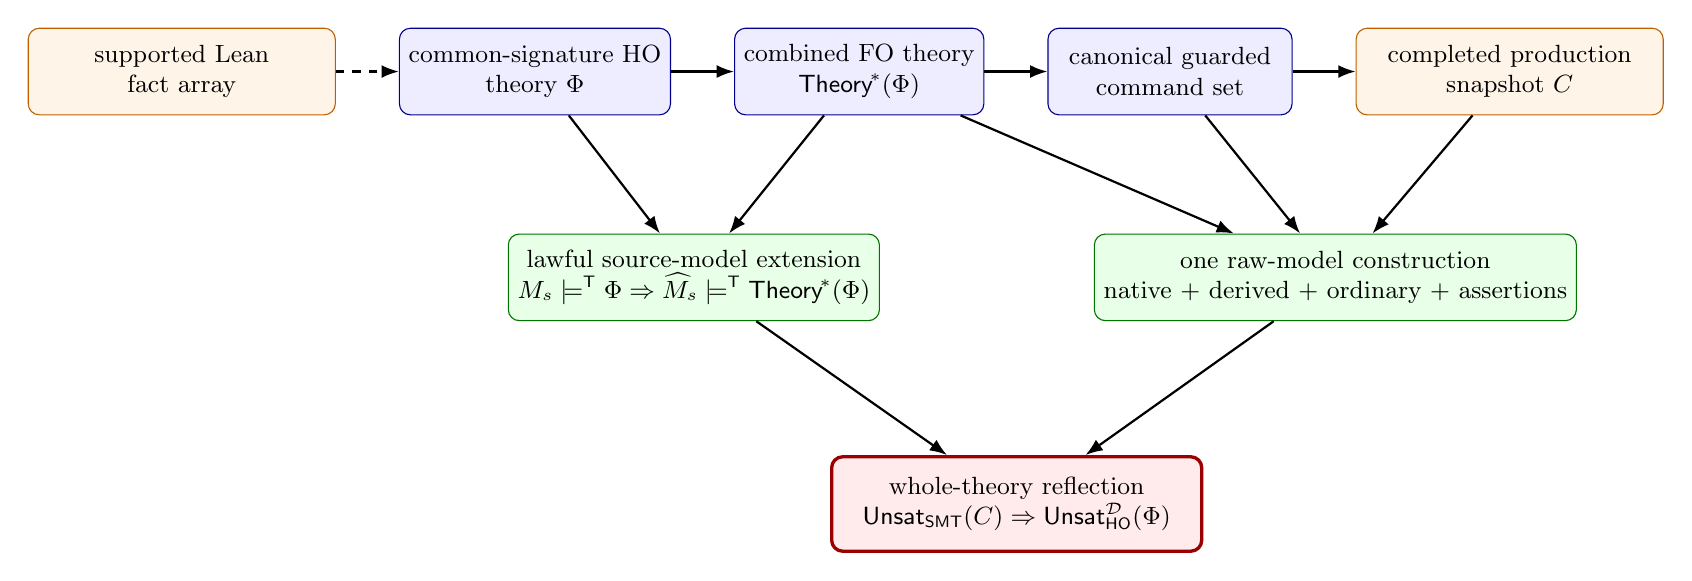
\begin{tikzpicture}[
  node distance=8mm and 8mm,
  every node/.style={font=\small,align=center},
  stage/.style={draw=blue!55!black,fill=blue!7,rounded corners,
    minimum width=31mm,minimum height=11mm},
  proof/.style={draw=green!45!black,fill=green!9,rounded corners,
    minimum width=39mm,minimum height=11mm},
  boundary/.style={draw=orange!75!black,fill=orange!9,rounded corners,
    minimum width=39mm,minimum height=11mm},
  final/.style={draw=red!60!black,fill=red!8,very thick,rounded corners,
    minimum width=47mm,minimum height=12mm},
  arrow/.style={-{Latex[length=2.2mm]},thick}
]
  \node[boundary] (lean) {supported Lean\\fact array};
  \node[stage,right=of lean] (ho) {common-signature HO\\theory $\Phi$};
  \node[stage,right=of ho] (fo) {combined FO theory\\$\Theorys{\Phi}$};
  \node[stage,right=of fo] (spec) {canonical guarded\\command set};
  \node[boundary,right=of spec] (prod) {completed production\\snapshot $C$};

  \node[proof,below=15mm of fo,xshift=-21mm] (model1) {lawful source-model extension\\
    $M_s\satt\Phi\Rightarrow\widehat M_s\satt\Theorys{\Phi}$};
  \node[proof,below=15mm of spec,xshift=21mm] (model2) {one raw-model construction\\
    native $+$ derived $+$ ordinary $+$ assertions};
  \node[final,below=17mm of model1,xshift=41mm] (final) {whole-theory reflection\\
    $\unsat_{\mathsf{SMT}}(C)\Rightarrow
      \unsat_{\mathsf{HO}}^{\mathcal D}(\Phi)$};

  \draw[arrow,dashed] (lean) -- (ho);
  \draw[arrow] (ho) -- (fo);
  \draw[arrow] (fo) -- (spec);
  \draw[arrow] (spec) -- (prod);
  \draw[arrow] (ho) -- (model1);
  \draw[arrow] (fo) -- (model1);
  \draw[arrow] (fo) -- (model2);
  \draw[arrow] (spec) -- (model2);
  \draw[arrow] (prod) -- (model2);
  \draw[arrow] (model1) -- (final);
  \draw[arrow] (model2) -- (final);
\end{tikzpicture}%
}
\caption{The current aggregate proof architecture. Datatype lawfulness and a
uniform guard interpretation parameterize the model construction. Command-set
agreement models production reordering and duplicate suppression exactly at the
membership-based raw semantics.}
\label{fig:proof-architecture}
\end{figure}

\subsection{What the composed theorem proves}

\begin{enumerate}[leftmargin=*]
 \item HO and FO syntax is intrinsically typed, and flattened
       defunctionalization is total on the complete modeled core.
 \item Every source fact contributes its translated body, closure equations,
       extensionality obligations, and declaration occurrences to one combined
       target theory over one signature.
 \item One canonical target model simultaneously satisfies that whole target
       theory whenever one source model satisfies the whole source theory.
 \item Productive monomorphic datatype blocks have finite free-algebra source
       semantics and exact native raw-command semantics.
 \item Guarded carrier relations preserve typed terms, equality, and both
       quantifiers; recursive datatype guards denote exactly the structural
       image of the source carrier.
 \item One induced raw model validates native datatype commands, simultaneous
       guard definitions, ordinary declarations, and every guarded assertion.
 \item Exact representation is semantic command-set equivalence. It therefore
       admits production interleaving and duplicate elimination without
       weakening or strengthening the model obligations.
 \item Common-environment reification retains the exact ordered Lean fact array,
       and fresh aggregate VCG retains an exact representation theorem.
 \item Production traces reconnect native and recursive-guard commands to the
       completed final snapshot. \texttt{TheoryAgreement.build?} checks the
       remaining whole-array command set and returns proof-producing evidence.
 \item Semantic unsatisfiability of the agreed completed snapshot reflects to
       unsatisfiability of the entire intrinsic source theory in every
       datatype-lawful source model.
\end{enumerate}

\subsection{Exact boundaries}

\begin{itemize}[leftmargin=*]
 \item No denotational semantics is postulated for arbitrary \texttt{Lean.Expr};
       the final proposition concerns the reified intrinsic theory.
 \item Semantic command unsatisfiability is a premise. Correctness of an
       external solver's reported \texttt{unsat} answer requires certificate
       replay or another independently checked argument.
 \item The live extensible translator does not automatically construct the
       shared encoding, native representation, static guard representation,
       uniform guard interpretation, or common aggregate reification witness.
       Production reflection applies once those proof objects and exact
       agreement are present.
 \item \texttt{TranslateState.status} is operational metadata; it cannot replace
       a \texttt{TheoryRepresentation} or \texttt{TheoryAgreement} witness.
 \item The live allocator is finite, while the intrinsic \texttt{SMT.Encoding}
       interface supplies total injections over the modeled symbol family. The
       current theorem takes that total encoding as an explicit representation
       premise rather than claiming it is extracted from every allocator state.
 \item Unsupported dependent syntax, indexed or nonproductive inductives,
       dependent or function-valued datatype fields, unsafe indirect recursion,
       unrestricted translation handlers, nonrecursive raw definitions, and
       native-HO commands remain outside the modeled theorem.
\end{itemize}

\section{Machine-checked theorem inventory}
\sectioncontents{The named results that implement the proof story.}

\begin{sloppypar}
\small
The principal declarations, in proof order, are:
\begin{enumerate}[leftmargin=*]
 \item \path{Datatype.ctor_inj}, \path{Datatype.ctor_ne},
       \path{Datatype.ctor_cases}, \path{Datatype.sel_ctor},
       \path{Datatype.test_ctor}, and \path{Datatype.Args.get_height_lt_ctor}:
       finite free-algebra datatype laws.
 \item \path{Datatype.Lawful.productive}: any lawful source datatype carrier
       supplies a productive intrinsic block.
 \item \path{Flattened.LambdaBody.denote_etaBody} and
       \path{Flattened.TargetArguments.completeApp_denote}: eta opening and one
       flattened application preserve repeated source application.
 \item \path{Flattened.translate_denote}: the translated term component has
       the source denotation in the canonical model.
 \item \path{Flattened.generated_valid}: all generated closure equations and
       extensionality formulas are valid in that same model.
 \item \path{Flattened.model_extension_theory}: one source model satisfying a
       finite theory extends to the combined flattened target theory.
 \item \path{Flattened.target_theories_unsat_implies_source_unsat}: combined FO
       unsatisfiability reflects to the complete finite HO theory.
 \item \path{SMT.encode_theories}: the pure encoder gives an exact semantic
       command-set representation of the combined theory.
 \item \path{SMT.Datatype.command_sound} and
       \path{SMT.Datatype.EnvRepresentation.native_valid}: one block and the
       complete dependency-ordered native prefix satisfy the raw datatype laws.
 \item \path{FO.FamilyTerm.guardDenote_rel}: related FO models preserve every
       term under guard-restricted quantifier semantics.
 \item \path{Datatype.Val.wf_iff_selWF}: the structural datatype image equals
       the tester/selector predicate emitted by production.
 \item \path{SMT.Datatype.wfDefs_valid}: exact mutual \texttt{wf\_T}
       definitions satisfy the raw simultaneous graph semantics.
 \item \path{SMT.guardTerm_rel_eval}: guard-aware raw evaluation agrees with
       denotation in any symbol-related target model.
 \item \path{SMT.guarded_lift}: native commands, derived definitions, ordinary
       declarations, and guarded assertions hold in one raw model.
 \item \path{SMT.representation_sound}: the unguarded complete representation
       has the corresponding one-model lifting theorem.
 \item \path{SMT.commands_unsat_implies_source_theory_unsat}: semantic
       raw-command unsatisfiability reflects to the lawful intrinsic HO theory.
 \item \path{Reification.reifyTheory?}: an exact Lean fact array reifies under
       one datatype environment and signature bridge without reordering.
 \item \path{VCG.theoryCommands_represents} and
       \path{VCG.guardedTheoryCommands_represents}: pure aggregate generation
       retains ordinary and guarded representation evidence.
 \item \path{VCG.runTheory_represents} and
       \path{VCG.runGuardedTheory_represents}: fresh stateful runs retain those
       exact aggregate representations.
 \item \path{VCG.TheoryStateRepresents.unsat_source} and
       \path{VCG.runGuardedTheory_unsat_implies_source_unsat}: the intrinsic
       stateful compositions reflect to source-theory unsatisfiability.
 \item \path{VCG.CertifiedDataEnv.Representation.theory_unsat}: one production
       datatype and guard package reflects any exactly represented finite
       source theory.
 \item \path{VCG.TheoryAgreement.unsat_source} and
       \path{VCG.TheoryAgreement.unsat_source_script}: the complete production
       snapshot, with optional leading logic command, reflects through checked
       whole-theory agreement.
\end{enumerate}
\end{sloppypar}

The earlier unary results---\path{fundamental},
\path{fundamental_sentence}, and the unary
\path{target_unsat_implies_source_unsat}---remain machine-checked as an
independent reference model.

\end{document}
